%%%%%%%%%%%%%%
%% Run LaTeX on this file several times to get Table of Contents,
%% cross-references, and citations.

%% If you have font problems, you may edit the w-bookps.sty file
%% to customize the font names to match those on your system.

%% w-bksamp.tex. Current Version: Feb 16, 2012
%%%%%%%%%%%%%%%%%%%%%%%%%%%%%%%%%%%%%%%%%%%%%%%%%%%%%%%%%%%%%%%%
%
%  Sample file for
%  Wiley Book Style, Design No.: SD 001B, 7x10
%  Wiley Book Style, Design No.: SD 004B, 6x9
%
%
%  Prepared by Amy Hendrickson, TeXnology Inc.
%  http://www.texnology.com
%%%%%%%%%%%%%%%%%%%%%%%%%%%%%%%%%%%%%%%%%%%%%%%%%%%%%%%%%%%%%%%%

%%%%%%%%%%%%%
% 7x10
%\documentclass{wileySev}

% 6x9
\documentclass{wileySix}

\usepackage{graphicx}

%%%%%%%
%% for times math: However, this package disables bold math (!)
%% \mathbf{x} will still work, but you will not have bold math
%% in section heads or chapter titles. If you don't use math
%% in those environments, mathptmx might be a good choice.

% \usepackage{mathptmx}

% For PostScript text
\usepackage{w-bookps}

%%%%%%%%%%%%%%%%%%%%%%%%%%%%%%%%%%%%%%%%%%%%%%%%%%%%%%%%%%%%%%%%
%% Other packages you might want to use:

% for chapter bibliography made with BibTeX
% \usepackage{chapterbib}

% for multiple indices
% \usepackage{multind}

% for answers to problems
% \usepackage{answers}

%%%%%%%%%%%%%%%%%%%%%%%%%%%%%%
%% Change options here if you want:
%%
%% How many levels of section head would you like numbered?
%% 0= no section numbers, 1= section, 2= subsection, 3= subsubsection
%%==>>
\setcounter{secnumdepth}{3}

%% How many levels of section head would you like to appear in the
%% Table of Contents?
%% 0= chapter titles, 1= section titles, 2= subsection titles, 
%% 3= subsubsection titles.
%%==>>
\setcounter{tocdepth}{2}

%% Cropmarks? good for final page makeup
%% \docropmarks

%%%%%%%%%%%%%%%%%%%%%%%%%%%%%%
%
% DRAFT
%
% Uncomment to get double spacing between lines, current date and time
% printed at bottom of page.
% \draft
% (If you want to keep tables from becoming double spaced also uncomment
% this):
% \renewcommand{\arraystretch}{0.6}
%%%%%%%%%%%%%%%%%%%%%%%%%%%%%%

%%%%%%% Demo of section head containing sample macro:
%% To get a macro to expand correctly in a section head, with upper and
%% lower case math, put the definition and set the box 
%% before \begin{document}, so that when it appears in the 
%% table of contents it will also work:

\newcommand{\VT}[1]{\ensuremath{{V_{T#1}}}}

%% use a box to expand the macro before we put it into the section head:

\newbox\sectsavebox
\setbox\sectsavebox=\hbox{\boldmath\VT{xyz}}

%%%%%%%%%%%%%%%%% End Demo


\begin{document}


\booktitle{Survey Methodology}
\subtitle{This is the Subtitle}

\authors{Robert M. Groves\\
\affil{Universitat de les Illes Balears}
Floyd J. Fowler, Jr.\\
\affil{University of New Mexico}
}

\offprintinfo{Survey Methodology, Second Edition}{Robert M. Groves}

%% Can use \\ if title, and edition are too wide, ie,
%% \offprintinfo{Survey Methodology,\\ Second Edition}{Robert M. Groves}

%%%%%%%%%%%%%%%%%%%%%%%%%%%%%%
%% 
\halftitlepage

\titlepage


\begin{copyrightpage}{2007}
Survey Methodology / Robert M. Groves . . . [et al.].
\       p. cm.---(Wiley series in survey methodology)
\    ``Wiley-Interscience."
\    Includes bibliographical references and index.
\    ISBN 0-471-48348-6 (pbk.)
\    1. Surveys---Methodology.  2. Social 
\  sciences---Research---Statistical methods.  I. Groves, Robert M.  II. %
Series.\\

HA31.2.S873 2007
001.4'33---dc22                                             2004044064
\end{copyrightpage}



\dedication{To my parents}

\begin{contributors}
\name{Masayki Abe,} Fujitsu Laboratories Ltd., Fujitsu Limited, Atsugi,
Japan

\name{L. A. Akers,} Center for Solid State Electronics Research, Arizona
State University, Tempe, Arizona

\name{G. H. Bernstein,} Department of Electrical and
Computer Engineering, University of Notre Dame, Notre Dame, South Bend, 
Indiana; formerly of
Center for Solid State Electronics Research, Arizona
State University, Tempe, Arizona 
\end{contributors}

\contentsinbrief
\tableofcontents
\listoffigures
\listoftables


\begin{foreword}
This is the foreword to the book.
\end{foreword}

\begin{preface}
This is an example preface.
This is an example preface.
This is an example preface.
This is an example preface.

\prefaceauthor{R. K. Watts}
\where{Durham, North Carolina\\
September, 2007}

\end{preface}


\begin{acknowledgments}
From Dr.~Jay Young, consultant from Silver Spring, Maryland, I received
the initial push to even consider writing this book. Jay was a constant
``peer reader'' and very welcome advisor durying this year-long process.


To all these wonderful people I owe a deep sense of gratitude especially now
that this project has been completed.
\authorinitials{G. T. S.}
\end{acknowledgments}

\begin{acronyms}
\acro{ACGIH}{American Conference of Governmental Industrial Hygienists}
\acro{AEC}{Atomic Energy Commission}
\acro{OSHA}{Occupational Health and Safety Commission}
\acro{SAMA}{Scientific Apparatus Makers Association}
\end{acronyms}

\begin{glossary}
\term{NormGibbs}Draw a sample from a posterior distribution
of data with an unknown mean and variance using Gibbs sampling.

\term{pNull}Test a one sided hypothesis from a numberically
specified posterior CDF or from a sample from the posterior

\term{sintegral}A numerical integration using Simpson's rule
\end{glossary}

\begin{symbols}
\term{A}Amplitude

\term{\hbox{\&}}Propositional logic symbol 

\term{a}Filter Coefficient

\bigskip

\term{\mathcal{B}}Number of Beats
\end{symbols}

\begin{introduction}

%% optional, but if you want to list author:

\introauthor{Catherine Clark, PhD.}
{Harvard School of Public Health\\
Boston, MA, USA}

The era of modern \index{microelectronics}\index{microelectronics!modern} 
began in 1958 with the invention of the
integrated circuit by J.~S.~Kilby
 of Texas Instruments \cite{kilby}.
His first chip is shown in Fig.~I. For comparison,
Fig.~I.2 shows a modern microprocessor chip, \cite{beren}.


This is the introduction.
This is the introduction.
This is the introduction.
This is the introduction.
This is the introduction.
This is the introduction.

\begin{equation}
ABC {\cal DEF} \alpha\beta\Gamma\Delta\sum^{abc}_{def}
\end{equation}


\begin{chapreferences}{3.}
\bibitem{zkilby}J. S. Kilby,
``Invention of the Integrated Circuit,'' {\it IEEE Trans. Electron Devices,}
{\bf ED-23,} 648 (1976).

\bibitem{zhamming}R. W. Hamming,
                 {\it Numerical Methods for Scientists and 
                 Engineers}, Chapter N-1, McGraw-Hill, 
                 New York, 1962.

\bibitem{zHu}J. Lee, K. Mayaram, and C. Hu, ``A Theoretical
               Study of Gate/Drain Offset in LDD MOSFETs''
                     {\it IEEE Electron Device Lett.,} {\bf EDL-7}(3). 152 
                     (1986).
\end{chapreferences}
\end{introduction}

\chapter{Installation}
\hspace{0,5in}Latex merupakan system pengaturan cara pengetikan dokumen. Latex adalah perangkat lunak yang dapat di download tanpa harus membayar. Sejarahnya, Donald Knuth (Standford University) mulai mengembangkan sistem pemrosesan dokumen yang disebut "\,Tex dan Metafont" pada tahun 1977. Knut mengungkapkan bahwa Tex merupakan sistem pengetikan dengan tujuan
untuk membuat buku yang "\,cantik" , khususnya yang terdiri atas formula-formula matematis. Hingga sekarang, Latex telah berkembang dan project saat ini adalah Latex3.\par \vspace{12pt}

LaTeX merupakan word processor (pengolah kata, pembuat dokumen) mirip Microsoft Word. LaTeX lebih cocok digunakan untuk membuat dokumen yang panjang, bukan yang pendek. Dengan begitu, keampuhan LaTeX dapat ditampilkan. LaTeX juga lebih dapat menampilkan kecanggihannya ketika kita menulis scientific document.
Kelebihan menggunakan latex antara lain :
1.  Hasil tampilan dokumennya profesional sekali dengan kata lain mirip buku teks.
2.  Ketika kita ngetik, kita tidak peduli tampilan dan layout. Layout nanti diatur oleh file utama (misal: main.tex).
3.  LaTeX itu free of charge atau gratis.
4.  Rumus-rumus matematika dapat diatur dengan mudah.
5.  Tidak pernah crash (adanya error karena salah memasukkan command atau karena software tidak updated)
6.  File-nya relatif kecil.
8.  Tutorial dan command untuk symbol banyak tersedia di internet

\hspace{0,3in}Biasanya Latex digunakan untuk mengetik dokumen yang berisi formula-formula matematis. Jenis dokumen yang dihasilkan dapat berupa artikel, buku, tesis, disertasi, hingga surat bisnis maupun surat pribadi. Dokumen yang hasilkan oleh latex berbeda antara input dengan output dari MS Word atau Libre Office. Misalnya di MS Word kita mengetik "\,\$a\$" maka yang muncul di dokumen hasil adalah "\,\$a\$", sedangkan dengan input yang sama, Latex memberikan output "\,a". Karena ide dari Latex adalah membiarkan penulis menulis dokumen dan menyerahkan desain dokumen ke "\,document designer", maka hasil dari dokumen Latex akan terlihat lebih "\,cantik".\par \vspace{12pt}

\section{Instalasi LaTeX}\par \vspace{8pt}

Ada banyak editor untuk latex dan tidak semua editor sesuai dengan setiap pengguna. Semua itu tergantung pada selera masing-masing. Karena alasan ini, akan saya tunjukan bagaimana dasar-dasar latex berjalan. Banyak pengguna memilih MikTeX untuk Windows karena MikTeX sudah mempunyai semuanya yang diperlukan untuk menjalankan program latex.
\par \vspace{12pt}
\subsection{Linux}
\par \vspace{8pt}
Jika menggunakan linux, maka Anda bisa menggunakan paket texlive di beberapa repository. Setelah itu Anda bisa menggunakan berbagai macam text editor dan menjalankan file dengan format .tex dengan perintah pdflatex.
\par \vspace{12pt}
\subsection{Windows}
\par \vspace{12pt}
Langkah pertama untuk pengguna windows yaitu :

\newcounter{numberedCntC}
\begin{enumerate}
\item Install tex compiler. Tex compiler yang sering digunakan yaitu Miktex dan Texlive. Kedua perangkat lunak ini merupakan software yang paling banyak digunakan meskipun banyak perangkat lunak yang lain. Miktex yang diinstall pertama kali hanya memiliki paket dasar saja. Kemudian paket-paket tambahan lainnya dapat diinstall sesuai kebutuhan. Berbeda dengan Texlive, saat menginstall Texlive maka semua paket yang
ada akan diinstal meskipun belum tentu kita butuhkan. Sehingga instalasi Texlive lebih lama (kurang lebih 20 menit pada komputer dengan processor pentium i3 dan RAM 6 GB) daripada Miktex. Pilihan Miktex atau Texlive tergantung dari ruang hardisk yang ada, jika ruang hardisk masih banyak tidak ada salahnya menginstall Texlive. Saat ini saya menggunakan Miktex
(OS Windows) dan Texlive (Unix). Keduanya dapat didownload di Miktex website dan Texlive website (pilih salah satu).
\item Install Tex Editor. Tex editor yang tidak berbayar juga banyak. Baik di windows maupun unix, bisa menggunakan texmaker sebagai tex editor. Perangkat lunak tersebut bisa di download melalui websitenya. Didalam texmaker inilah nantinya untuk menulis dokumen latex.
\item Langkah terakhir yaitu memulai menggunakan latex. Buka texmaker, pilih file kemudian pilih new, kemudian tulis seperti contoh dibawah ini:
\setcounter{numberedCntC}{\theenumi}
\end{enumerate}

\ref{image1.jpg}:
\begin{figure}[ht]
	\centerline{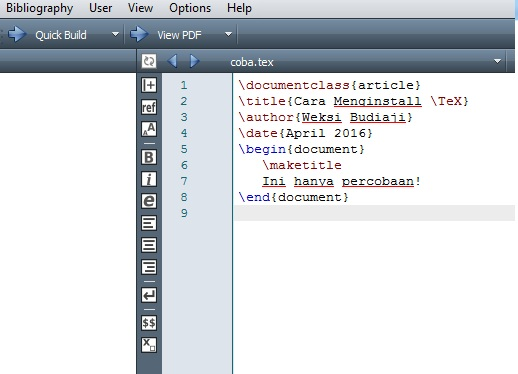
\includegraphics[width=13.54cm,height=9.78cm]{gambar/image1.jpg}}
\caption{Texmaker}
\label{image1.jpg}
\end{figure}

\begin{enumerate}
\setcounter{enumi}{\thenumberedCntC}
\item Setelah menulis file latex seperti diatas, maka save file. Misalkan save dengan nama 'coba'. Kemudian klik tanda panah "\,quick build" atau bisa dengan tekan tombol F6. Untuk melihat hasil pdf nya bisa dengan menekan tombol F7.
\setcounter{numberedCntC}{\theenumi}
\end{enumerate}

\textbf{Macam- macam Editor Latex}

\newcounter{numberedCntE}
\begin{enumerate}
\item \textbf{Emacs dengan AUCTex}
\begin{itemize}
\item OS: Windows, Mac (termasuk fork Aquamacs), Unix
\item Lisensi: Free software (GPL)
\item Bahasa: de, dk, fr, is, it, jp, nl, pl, se, sk didukung oleh AUCTeX
\item Unicode: Ya, sejak Emacs 23
\item RTL/bidirectional support: sejak Emacs 24, melalui bidi-mode
\item \% !TeX directives: Tidak, tetapi Emacs memiliki beberapa realisasi untuk file local variables
\item Syntax highlighting: Ya, bisa diatur lewat customize and Elisp
\item Code completion: Ya, via Emacs Predictive Completion, yang mendukung AUCTeX tanpa konfigurasi lebih lanjut
\item Code folding: Ya
\item Spell checking: Ya
\item SyncTeX: Ya
\item Built-in output viewer: Ya
\item Project management: org-mode, reftex-mode
\end{itemize}
\hspace{0,5in}Emacs adalah salah satu editor tertua, yang mendukung mode penyuntingan LaTeX, ConTeXt, dan Plain TeX, AUCTeX dan paket untuk mengelola kode-kode sumber, RefTeX.

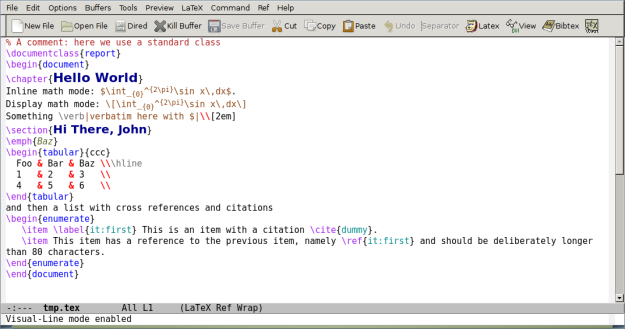
\includegraphics[width=10.95cm,height=7.87cm]{gambar/image2.jpg}
\par \vspace{12pt}

RefTeX membuat seluruh referensi Anda mudah ditemukan layaknya C-c $<$key$>$, baik untuk BibTeX maupun biblatex, dan ia memiliki pintasan (shortcut key) pula untuk bernavigasi di antara bagian-bagian dokumen dengan menggunakan C-c =: secara default.


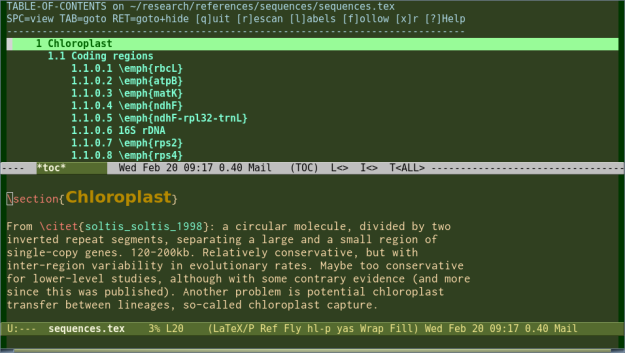
\includegraphics[width=15.64cm,height=8.83cm]{gambar/image3.jpg}

(Tema warna dapat dikonfigurasi sebebas mungkin)

AUCTeX mendukung multi-file parsing, sehingga dokumen-dokumen besar dengan perintah \textit{$\setminus$input} atau \textit{
$\setminus$include} mudah dikompilasikan dengan \textit{C-c C-c} pada berkas yang bersangkutan. Tidak perlu lagi kembali ke master file hanya untuk mengompilasi.
\par \vspace{12pt}
Fitur AUCTeX \textit{preview-latex} adalah pratayang WYSIWYG untuk rumus-rumus. Fitur-fitur terkemuka Emacs:

\begin{itemize}
\item Menggunakan table-insert bersama dengan fungsi
table-generate-source dan table-recognize-* untuk membuat tabel-tabel dengan mudah.
\item Banyak sekali shortcut key tersedia
\item Terdokumentasi dengan baik, baik Emacs itu sendiri melalui manual Emacs dan manual AUCTex Texinfo, maupun melalui banyak buku dalam beberapa bahasa.
\end{itemize}

\item \textbf{Vim dengan LaTeX-suite}
\begin{itemize}
\item OS: Windows, Mac, Linux, BSD, dan lain-lain
\item Lisensi: Open Source Charityware
\item Bahasa: ?
\item Unicode: Ya
\item RTL/bidi support: sebagian
\item \% !TEX directives: Tidak, tetapi memiliki modelines
\item Syntax Highlighting: Ya, bisa dikustomisasi
\item Code Completion: Ya (menggunakan Omni Completion, bisa diperluas dengan plugin SnipMate)
\item Code Folding: Ya
\item Spell Checking: Ya
\item SyncTeX: Ya, lihat pertanyaan ini
\item Built-in Output Viewer: Tidak
\item Project Management: ?
\item Jika Anda benar-benar kelas berat, Anda akan selalu menggunakan Vim. Ada banyak macro yang dibuat untuk Vim untuk membantu menyunting berkas LaTeX.
\end{itemize}
\begin{figure}[ht]

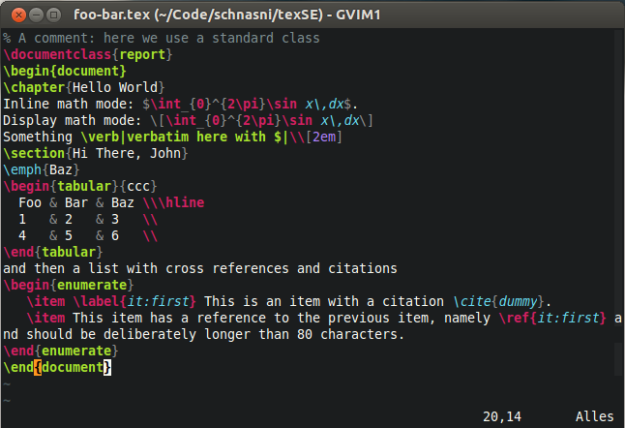
\includegraphics[width=15.57cm,height=10.66cm]{gambar/image4.jpg}
\end{figure}

Anda dapat melakukan word/command completion melalui
\begin{equation}
<C-P> dan <C-N>,
\end{equation}untuk memilih saran sebelumnya atau sesudahnya.

Ada versi Vim dengan menu-menu grafis, yang bernama gVim. Jika ia digunakan dengan Latex-suite, maka banyak perintah TeX ditampilkan di menubar untuk mempercepat penyuntingan.
\par \vspace{12pt}
\textbf{Fitur-Fitur}
\par \vspace{12pt}
Vim juga memiliki fitur code-folding, karena paket vim-late menawarkan code-folding otomatis. Folding juga bisa dilakukan secara manual berdasarkan kunci (misalnya \{\{\{ dan \}\}\}) untuk membuka dan menutup fold otomatis. Contoh folds bisa dilihat pada gambar berikut:

\begin{figure}[ht]

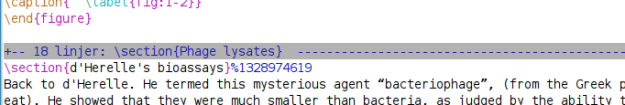
\includegraphics[width=15.12cm,height=2.54cm]{gambar/image5.jpg}
\end{figure}

Fitur Vim masih sangat banyak. Namun di dalam tulisan ini, yang bisa disebutkan adalah:

VIM

Regex

\begin{itemize}
\item Perintah dan pintasan kibor yang powerful
\item Sangat bisa dikustomisasi
\item Smart Indenting
\end{itemize}
LaTeX-Suite

\begin{itemize}
\item Panggil cepat kompiler dengan $\setminus$ll; tayangkan hasil dengan $\setminus$lv
\item Environments dapat diakses dengan tiga huruf dalam insert mode:
\end{itemize}
\hspace{0,2in}EEQ = environment persamaan

EFI = environment gambar (figure)

\begin{itemize}
\item Place-holders ($<$+text+$>$) dapat dilompati dengan Ctrl-J tanpa meninggalkan insert mode
\item Inverse searching: klik ganda penampil PDF dan Anda lompat ke baris kode sumber tex yang bersesuaian.
\end{itemize}

\item \textbf{Texmaker - texmaker}
\begin{itemize}
\item Platforms: Windows XP/Vista/7/8, OS X 10.5+, Linux
\item License: GPL, gratis
\item Languages: cs, de, el, en, es, fa, fr, gl, hu, it, nl, pl, pt, pt (bra), ru, se, sr, zh (cn), zh (tw)
\item Unicode: Ya
\item RTL/bidi: ?
\item \% !TEX directives: Tidak
\item Syntax Highlighting: Ya, bisa dikustomisasi
\item Code Completion: Ya, bisa dikustomisasi
\item Code Folding: Ya
\item Spell Checking: Ya
\item SyncTeX: Ya
\item Built-in Output Viewer: Ya, mendukung PDF
\end{itemize}
\item \textbf{TeXworks - texworks}
\begin{itemize}
\item OS: Windows XP/Vista/7/8, OS X, Linux
\item Lisensi: GPL
\item Bahasa: en, af, ar, ca, cs, de, fa, fo fr, it, ja, nl, ko, pl, pl, ru, sl, tr zh
\item Unicode: Ya
\item RTL/bidi: Ya
\item \% !TEX directives: Ya
\item Syntax Highlighting: Ya, regex-based
\item Code Completion: Ya, bisa dikustomisasi berdasarkan daftar 'known entry'
\item Code Folding: Tidak
\item Spell Checking: Ya, tetapi harus diinstal sendiri
\item SyncTeX: Ya
\item Built-in Output Viewer: Ya, PDF (Poppler-based)
\item Project Management: Tidak
\item Di Windows dan Linux, saya menggunakan TeXworks, yang menyediakan jendela editor kode dan pratayang. Klik pada pratayang dokumen akan langsung menandai kode LaTeX yang bersesuaian.
\end{itemize}

\item \textbf{Kile - kile}
\begin{itemize}
\item OS: Linux, Windows1 (XP, Vista, 7)
\item LIsensi: GNU GPL 2
\item Bahasa:
\begin{verbatim}bg, bs, ca, cs, da, de, el, en\_GB, eo, es, et, fi, fr, ga, gl, hi, hne, hu, it, ja, kk, lt, mai, ms, nb, nds, nl, nn, pl, pt, pt\_BR, ro, ru, sk, sv, tr, ug, uk, zh\_CN, zh\_TW
\end{verbatim}
\item Unicode: Ya
\item RTL/bidi: Ya
\item \% !TEX directives: Tidak2
\item Syntax Highlighting: Ya, bisa dikustomisasi
\item Code Completion: Ya, bisa dikustomisasi
\item Code Folding: Ya
\item Spell Checking: Ya
\item SyncTeX: Ya (namun flag -synctex=1 harus ditambahkan secara manual pada build engine)
\item Built-in Output Viewer: Terbatas3 (pratayang PNG dari sebagian kode - misalnya environment yang dipilih - dikonversikan dari DVI/PS/PDF)
\item Project Management: Ya
\end{itemize}
\begin{figure}[ht]

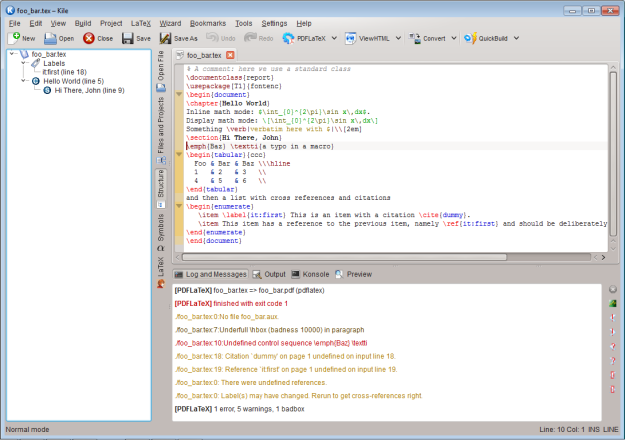
\includegraphics[width=14.76cm,height=10.39cm]{gambar/image6.jpg}
\end{figure}


\item \textbf{TeXstudio - texstudio}

\begin{table}[ht]
	\caption{Instalasi Paket}
	\centering
	\begin{tabular}{cccc}
		\hline
		No&Keterangan&\\
		\hline
		.1&OS: Windows XP/Vista/7, OS X, Linux, FreeBSD&\\
		.2&Lisensi: GPL v2&\\
		.3&Bahasa: cs, de, en, es, fr, hu, ja, pt\_BR, zh\_CN&\\
		.4&Unicode: Ya&\\
		.5&RTL/bidi: ?&\\
		.6&TeX directives: Ya&\\
		.7&Syntax Highlighting: Ya, bisa dikustomisasi&\\
		.8&Code Completion: Ya, bisa dikustomisasi dan auto-customized&\\
		.9&Unicode: Ya&\\
		.10&Code Folding: Ya&\\
		.11&Spell Checking: Ya&\\
		.12&SyncTeX: Ya&\\
		.13&Built-in Output Viewer: Ya, mendukung PDF&\\
		.14&Project Management: Ya&\\
		.15&Saya merekomendasikan TeXstudio sebagai fork yang menarik dari Texmaker yang saya rasa lebih nyaman dan bisa dikustomisasi.&\\
		\hline
	\end{tabular}
\end{table}
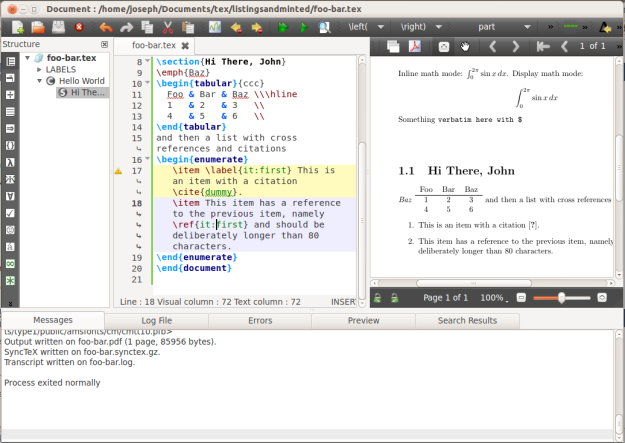
\includegraphics[width=15.23cm,height=10.79cm]{gambar/image7.jpg}

Fitur-fitur lainnya:
\begin{itemize}
\item cross-platform
\item dukungan penulisan (incremental search, folding, navigasi, auto-completion, custom macros)
\item syntax highlighting
\item inline interactive spell-checking
\item mendukung program-program LaTeX utama, termasuk tikz, pstricks, dan lain-lain
\item multi-views: math, structure
\item dukungan SVN
\item bisa berjalan via USB flash disk
\item mendukung synctex
\item termasuk penampil PDF, tetapi masih bisa dikonfigurasi untuk memakai viewer eksternal (juga dengan synctex)
\item developer dan komunitas yang sangat aktif dan responsive
\end{itemize}


\item \textbf{LyX}
\begin{itemize}
\item OS: Windows, Mac, and Linux
\begin{itemize}
\item Lisensi: Open Source
\item Sangat intuitif dan ramah pengguna, dan bisa impor/ekspor ke LaTeX.
\item Terlalu banyak ftur untuk disebutkan, paling bagus: Jika Anda ingin menulis rumus matematika "\,2-dimensional", LyX cocok untuk itu.
\end{itemize}
\end{itemize}
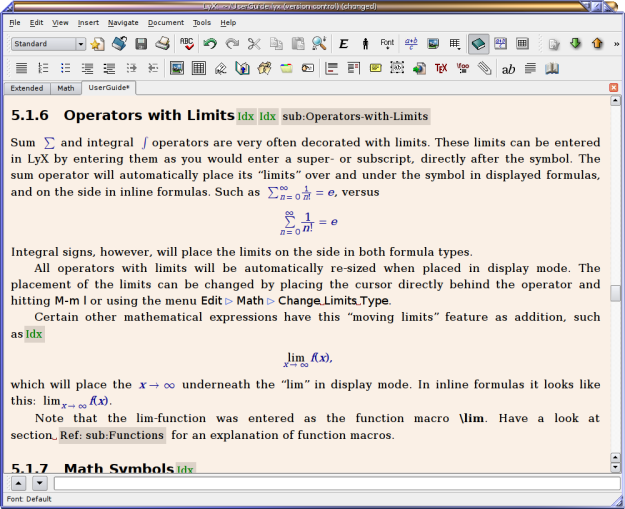
\includegraphics[width=14.10cm,height=11.48cm]{gambar/image8.jpg}

\item \textbf{Sublime Text dengan LaTeX Plugin}
\setcounter{numberedCntE}{\theenumi}
\hspace{0,2in}OS: Windows, Mac, Linux

Ini adalah editor yang sederhana tetapi powerful. Sublime Text mirip Notepad++, tetapi tersedia untuk banyak platform dan sangat mudah diatur untuk LaTeX dengan plugin LaTeXTools atau LaTeXing -keduanya tersedia dari Package Control. Sublime juga mirip TextMate, tetapi dikembangkan lebih aktif dan memiliki komunitas yang besar yang menyediakan plugin-nya. Sublime juga lebih cantik daripada keduanya.
\par \vspace{12pt}

Perhatikan bahwa ini adala software berbayar, dan meminta lisensi selama periode evaluasi (seharga USD 70). Dimungkinkan untuk menjalankan Sublime Text tanpa membeli lisensi, tetapi Anda akan terus diingatkan bahwa Anda menggunakan salinan yang belum diregistrasikan.
\par \vspace{12pt}


Sublime Text memiliki peralatan yang canggih untuk mengetik, yang Anda tidak mau tinggalkan ketika bekerja dengannya:

\begin{itemize}
\item multiple cursors
\item go-to ke mana saja
\item snippets
\item incremental find
\item manajemen proyek
\item build-systems yang banyak
\end{itemize}
dan banyak lagi (lihat Perfect Workflow in Sublime Text 2). Skrinsot di bawah juga menampakkan fiturnya untuk menemukan sitas-sitasi (citations) dari BibTeX.
\par \vspace{12pt}

Sublime Text ini editor yang hampir sempurna, dengan potensi yang hampir tidak terbatas. Daftar fiturnya panjang sekali. Instal Package Manager, dan paket-paket tambahan dari repositori bisa dipasang dalam beberapa detik saja.

\begin{itemize}
\item OS: Windows, Unix
\item Lisensi: Free to try, free to buy
\item \% !TEX directives: Ya
\item Syntax highlighting: Ya
\item Code completion: Ya
\item Code folding: Ya
\item Spell check: Ya, baik built-in maupun dengan plugin
\item SyncTeX: Ya
\item Built-in output viewer: Tidak
\item Project management: Ya
\end{itemize}
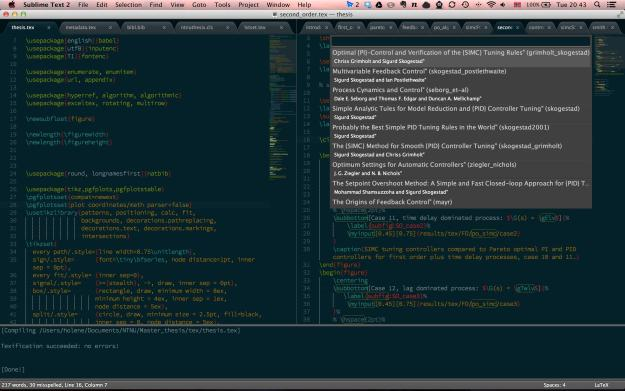
\includegraphics[width=15.67cm,height=9.80cm]{gambar/image9.jpg}

\item \textbf{TeXlipse}
\begin{itemize}
\item OS: Windows, Mac, Linux and others (Java based)
\item Lisensi: Open Source
\end{itemize}
Saya telah berbahagia menggunakan TeXlipse di Eclipse sejak lama, ia memiliki code completion terintegrasi (termasuk entri-entri BibTeX), templat-templat yang mudah dikustomisasi, panel outline, dan secara langsung ia terintegrasi dengan Eclipse itu sendiri yang secara otomatis memiliki shortcuts, version control, dan lain-lain.
\par \vspace{12pt}

Ada plugin penampil PDF untuk Eclipse bernama Pdf4Eclipse dengan dukungan SyncTeX, yang mendukung pencarian maju/mundur di dalam dokumen LaTeX. Karena TeXlipse me-rebuild kode-kode LaTeX secara otomatis (di background) setelah sekali disimpan, maka kode dan pratayang dari dokumen selalu disinkronkan.

\item \textbf{Gummi}
\begin{itemize}
\item OS: Linux (tersedia versi unstable untuk Windows)
\item Lisensi: Open Source
\end{itemize}


Emacs bagus, tetapi yang seringkali saya pakai adalah Gummi. Ia memiliki panel pratayang yang sangat berguna untuk mengetahui kesalahan sintaks dan kesalahan format sesegera mungkin. Plus, ketika Anda menyimpan dokumen LaTeX ia akan menyimpan PDF secara otomatis. Fitur lainnya termasuk peralatan bantuan penulisan matriks, memasukkan gambar, dan
sitasi (citation).
\par \vspace{12pt}

\begin{figure}[ht]

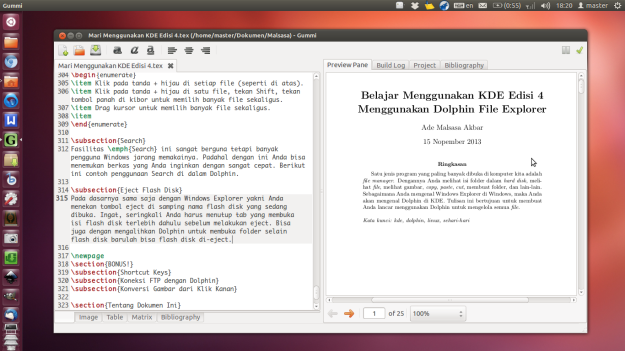
\includegraphics[width=15.45cm,height=8.68cm]{gambar/image10.jpg}
\end{figure}

\item \textbf{LaTeXila}
\begin{itemize}
\item OS: Linux
\item Lisensi: Open source
\item Unicode: Ya
\end{itemize}
\hspace{0,5in}LaTeXila adalah lingkungan LaTeX terintegrasi untuk GNOME. Ia memiliki antarmuka yang bagus dan jelas. Ia tersedia di Ubuntu Software Center. Anda dapat melihat preview dari apa yang Anda tulis kapanpun Anda mau.
\par \vspace{12pt}

LaTeXila memiliki komentar-komentar "\,ajaib" untuk membuat todonotes, yang akan tayang di panel struktur di sebelah kiri. Komentar itu adalah \%TODO dan \%FIXME, yang harus diikuti oleh teks (jika tidak ada teks, maka tidak ada yang tayang di panel).

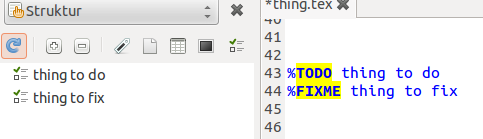
\includegraphics[width=12.78cm,height=3.68cm]{gambar/image11.jpg}


\item \textbf{Geany with GeanyLaTeX}
\begin{itemize}
\item OS: Windows, Mac, Linux dan lain-lain
\item Lisensi: Open Source
\end{itemize}
\end{enumerate}


Editor bagus lainnya adalah Geany. Software ini memiliki plugin untuk LaTeX. Plugin ini di-maintain oleh salah satu developer utama Geany sendiri. Plugin ini memiliki wizard untuk dokumen LaTeX baru, autocompletion, insert environment dengan mudah, dan tentu terdokumentasi dengan baik.



\chapter{Your First Document}
\section {Pengertian Latex}\par



TEX merupakan perangkat lunak pengolah dokumen yang terutama ditujukan menghasilkan dokumen yang berisi simbol-simbol matematik. TEX diciptakan oleh Donald E. Knuth (Mei1977) sebaga ibahasa pembentuk dokumen (document formatting language). LaTeX adalah sistem typesetting yang dapat digunakan untuk membuat artikel, buku, surat, dan publikasi lain berkualitas tinggi. LaTeX berbasiskan pada TeX, bahasa typesetting aras bawah yang didesain oleh Donald E. Knuth. LaTeX tidak bekerja seperti pengolah kata WYSIWYG (what you see is what you get), jenis persiapan dokumen yang sudah banyak dipakai oleh banyak orang. Dengan LaTeX, Anda tidak harus perduli dengan pemformatan dokumen dan tidak perlu mengatur rapi untuk penulisan teks sendiri, hanya tentang penulisan dokumen.


\ref{latex.jpg}:
\begin{figure}[ht]
	\centerline{
\includegraphics[width=10cm,height=7cm]{gambar/latex.jpg}}
	\caption{Latex}
	\label{latex.jpg}
\end{figure}

Perangkat lunak TEX memiliki kemampuan yang baik untuk mengolah dokumen-dokumen yang berkualitas tinggi. Kelemahannya, perintah perintahnya sulit digunakan untuk menuliskan dokumen terstruktur yang terdiri dari unsur-unsur bab, sub-bab, paragraph, table dan gambar bernomor, dsb.\par 
\vspace{12pt}

Versi LATEX yang sudah baku ini memiliki beberapa kekuatan, diantaranya adalah:

\begin{itemize}
\item Standard yang sangat baik untuk menyiapkan tulisan teks,formula 
teknis, dan tabel-tabel
\item Kemudahan penggunaan oleh penulis naskah.
\item Portabilitas dokumen pada berbagai platform
\item Adaptabilitas terhadap banyak bahasa (multilingual support)
\item Ketersediaan secara meluas dan bebas
\item Penulisan menjadi baik dan terstruktur rapi.
\item jenis Matematis dapat dituliskan dengan mudah.
\end{itemize}
\hspace{0,5in}Sebuah dokumen LATEX memiliki struktur yang dicirikan dengan blok yang diapit oleh pasangan perintah $\setminus$begin dan $\setminus$end. 
Untuk menyatakan jenis dokumen yang akan diolah, setiap dokumen harus dimulai dengan perintah:\par \vspace{12pt} $\setminus$documentclass\{\ldots \}\par \vspace{12pt}


Membuat dokumen dengan latex sangat sederhana. Anda bisa memulai membuat dokumen latex dengan mengetikan kode latex lalu ditambah dengan konten yang sederhana yaitu teks. Latex menggunakan kode-kode perintah yang terkontrol yang nantinya akan menentukan seperti apa hasil akhir dari dokumen yang anda buat. Setelah anda mengetikan kode-kode perintah latex, maka compiler dari editor latex dapat mengkompilasinya menjadi file .pdf. \par \vspace{12pt} 


\begin{table}[ht]
	\caption{Instalasi Paket}
	\centering
	\begin{tabular}{cccc}
		\hline
		No&Kelebihan&Kekurangan&\\
		\hline
		1.&Cocok untuk programmer&tidak user friendly seperti ms word&\\
		2.&Filenya relatif kecil&Harus hafal command&\\
		3.&Hasil tampilan dokumen profesional& Cocok untuk data skala besar&\\
		\hline
	\end{tabular}
\end{table}

\subsection {Kelas Dokumen}\par
\vspace{12pt}
Jenis dokumen yang akan diolah ditentukan oleh perintah pertama dalam bentuk: \par \vspace{12pt} $\setminus$documentclass$[$option$]$\{class\}\par \vspace{12pt}

Dalam perintah diatas,"\,class"dapat diganti oleh article, report, book, atau slides untuk menuliskan artikel, laporan, buku, atau transparansi untuk seminar. Sedangkan pada bagian"\,option" dapat dituliskan satu 
atau beberapa pilihan berikut : 10pt, 11pt, 12pt untuk menyatakan ukuran font utama yang digunakan didalam dokumen A4 paper, letterpaper menyatakan ukuran kertas yang digunakan titlepage, notitlepage untuk menyatakan apakah halaman judul akan dibuat terpisah dari badan dokumen atau tidak twocolumn untuk menampilkan dokumen dalam bentuk dua kolom twoside, oneside untuk menyatakan apakah dokumen akan dicetak pada satu 
sisi atau dua sisi dari kertas. contoh dasar menggunakan kode perintah dalam latex yaitu:\par \vspace{12pt}

$\setminus$documentclass\{article\}\par \vspace{12pt}

$\setminus$begin\{document\}\par \vspace{12pt}

Hello World!\par \vspace{12pt}

$\setminus$end\{document\}\par \vspace{12pt}

Kode diatas jika di compile maka akan muncul tulisan "\,Hello World!" 
dalam bentuk file .pdf.\par \vspace{12pt}

\textbf{Perintah-Perintah LATEX}

\newcounter{numberedCntB}
\begin{enumerate}
\item \textbf{Spasi dalam Latex}
\setcounter{numberedCntB}{\theenumi}
\end{enumerate}
Ada perintah khusus untuk membuat spasi dengan panjang tertentu baik secara horizontal maupun vertikal, yaitu :

\begin{itemize}
\item Jika ingin membuat jarak dengan panjang tertentu antara 2 baris, dapat menggunakan tanda ' $\setminus$$\setminus$ ' di akhir baris. Dan juga dapat menentukan sendiri panjang baris kosong dengan menggunakan perintah seperti contoh berikut ini :
\end{itemize}
\hspace{0,2in}baris 1 $\setminus$$\setminus$

$\setminus$vspace\{2cm\}

baris 2 $\setminus$$\setminus$

\par \vspace{12pt}

Dengan perintah ini, Latex akan mengosongkan baris-baris sepanjang 2 cm. Tanpa menggunakan perintah ini untuk membuat spasi dalam teks dokumen, Latex akan tetap menganggapnya 1 spasi.

\begin{itemize}
\item Jika ingin membuat spasi sejauh beberapa centimeter antara 2 kata dibutuhkan perintah sebagai berikut :
\end{itemize}
\hspace{0,5in}kata 1 $\setminus$hspace\{2cm\} kata 2\par \vspace{12pt}

Dengan perintah ini, Latex akan membuat spasi sejauh 2 centimeter.

Jadi, secara umum aturan yang dapat dipakai adalah akhiri paragraf dengan tanda ' $\setminus$$\setminus$ ' dan berikan 1 baris kosong antara tiap-tiap paragraf dan 1 spasi kosong antara masing-masing kata.

\begin{enumerate}
\setcounter{enumi}{\thenumberedCntB}
\item \textbf{Alignment dalam Latex}
\setcounter{numberedCntB}{\theenumi}
\end{enumerate}
\hspace{0,5in}Alignment/perataan baris pada Latex merupakan fitur untuk mengatur perataan teks yang terbagi menjadi rata kiri, rata kanan, atau rata tengah. Semua dokumen dalam Latex secara default diatur memiliki perataan justified (rata kanan kiri).

\begin{itemize}
\item Jika ingin mengatur dokumen rata kiri digunakan perintah sebagai berikut :
\end{itemize}
\hspace{0,5in}$\setminus$begin\{raggedright\}

\hspace{0,5in}isi dokumen yang diatur dengan rata kiri

\hspace{0,5in}$\setminus$end\{raggedright\}

\begin{itemize}
\item Jika ingin mengatur dokumen rata kanan digunakan perintah sebagai berikut :
\end{itemize}
\hspace{0,5in}$\setminus$begin\{raggedleft\}

\hspace{0,5in}isi dokumen yang diatur dengan rata kanan

\hspace{0,5in}$\setminus$end\{raggedleft\}

\begin{itemize}
\item Jika ingin mengatur dokumen rata tengah digunakan perintah sebagai berikut :
\end{itemize}
\hspace{0,5in}$\setminus$begin\{center\}

\hspace{0,5in}isi dokumen yang diatur dengan rata tengah

\hspace{0,5in}$\setminus$end\{center\}

\begin{enumerate}
\setcounter{enumi}{\thenumberedCntB}
\item \textbf{Bahasa dalam Latex}
\setcounter{numberedCntB}{\theenumi}
\end{enumerate}
\hspace{0,5in}Latex dapat menggunakan tulisan mengikuti aturan ejaan yang dimiliki bahasa tertentu. Kemampuan ini diatur oleh babel package. Mengubah peraturan bahasa dengan menggunakan babel akan secara otomatis mengubah nama-nama dari unit struktur dokumen (misalnya Abstract, Chapter, Index) 
menjadi terjemahannya.\par \vspace{12pt}

Perintah yang mengatur latex untuk menggunakan babel bahasa Indonesia seperti berikut :

$\setminus$dokumenclass \{a4paper, 12pt\}\{report\}\par \vspace{12pt}

$\setminus$usepage$[$bahasa$]$\{babel\}\par \vspace{12pt}

$\setminus$begin\{document\}\par \vspace{12pt}

. . . . . . . . . . . . . . . . . . . . .

. . . . . . . . . . . . . . . . . . . . .
\par \vspace{12pt}
$\setminus$end\{document\}

\begin{enumerate}
\setcounter{enumi}{\thenumberedCntB}
\item \textbf{Keterangan dalam Latex}
\setcounter{numberedCntB}{\theenumi}
\end{enumerate}
\hspace{0,5in}Jika Anda ingin menambahkan keterangan pada file yang tidak ingin tercetak, caranya adalah dengan menambahkan tanda \% diawal setiap baris keterangan. Contoh :\par \vspace{12pt}

$\setminus$dokumenclass \{a4paper, 12pt\}\{report\}\par \vspace{12pt}

$\setminus$usepage$[$bahasa$]$\{babel\}\par \vspace{12pt}

$\setminus$begin\{document\}\par \vspace{12pt}

ini baris keterangan, baris ini tidak akan tercetak dalam file 
keluaran

. . . . . . . . . . . . . . . . . . . . .\par \vspace{12pt}

$\setminus$end\{document\}

\begin{enumerate}
\setcounter{enumi}{\thenumberedCntB}
\item \textbf{Font dalam Latex}
\setcounter{numberedCntB}{\theenumi}
\end{enumerate}
Ada 3 jenis fonts dalam Latex :

\begin{itemize}
\item Roman. Cara menggunakannya seperti dibawah ini :
\end{itemize}
\hspace{0,5in}\{$\setminus$rmfamily teks yang ingin diformat \}

\begin{itemize}
\item Sans serif. Cara menggunakannya seperti dibawah ini :
\end{itemize}
\hspace{0,5in}\{$\setminus$sffamily teks yang ingin diformat \}

\begin{itemize}
\item Typewriter. Cara menggunakannya seperti dibawah ini :
\end{itemize}
\hspace{0,5in}\{$\setminus$ttfamily teks yang ingin diformat \}\par \vspace{12pt}



Ada 4 bentuk font dalam Latex :

\begin{itemize}
\item Italic. Cara mengaturnya sebagai berikut :
\end{itemize}
\hspace{0,5in}\{$\setminus$itshape teks yang ingin diformat \}

\begin{itemize}
\item Slanted. Cara mengaturnya sebagai berikut :
\end{itemize}
\hspace{0,5in}\{$\setminus$slshape teks yang ingin diformat \}

\begin{itemize}
\item Vertical. Cara mengaturnya sebagai berikut :
\end{itemize}
\hspace{0,5in}\{$\setminus$upshape teks yang ingin diformat \}

\begin{itemize}
\item SMALL CAPS. Cara mengaturnya sebagai berikut :
\end{itemize}
\hspace{0,5in}\{$\setminus$scshape teks yang ingin diformat \}
\par \vspace{12pt}


Ukuran Font

Ada beberapa macam ukuran font dalam Latex. Untuk menggunakan 
ukuran-ukuran tersebut, cara yang dapat digunakan adalah sebagai berikut :

\begin{itemize}
\item Tiny
\end{itemize}
\hspace{0,5in}\{$\setminus$tiny teks yang ingin diformat \}

\begin{itemize}
\item Scriptsize
\end{itemize}
\hspace{0,5in}\{$\setminus$scriptsize teks yang ingin diformat \}

\begin{itemize}
\item Footnotesize
\end{itemize}
\hspace{0,5in}\{$\setminus$footnotesize teks yang ingin diformat \}

\begin{itemize}
\item Small
\end{itemize}
\hspace{0,5in}\{$\setminus$small teks yang ingin diformat \}

\begin{itemize}
\item Normal
\end{itemize}
\hspace{0,5in}\{$\setminus$normalsize teks yang ingin diformat \}

\begin{itemize}
\item Large
\end{itemize}
\hspace{0,5in}\{$\setminus$large teks yang ingin diformat \}

\begin{itemize}
\item Larger
\end{itemize}
\hspace{0,5in}\{$\setminus$Large teks yang ingin diformat \}

\begin{itemize}
\item Largest
\end{itemize}
\hspace{0,5in}\{$\setminus$LARGE teks yang ingin diformat \}

\begin{itemize}
\item Huge
\end{itemize}
\hspace{0,5in}\{$\setminus$huge teks yang ingin diformat \}

\begin{itemize}
\item Huger
\end{itemize}
\hspace{0,5in}\{$\setminus$Huge teks yang ingin diformat \}

\begin{enumerate}
\setcounter{enumi}{\thenumberedCntB}
\item \textbf{Struktur Dasar Sebuah Dokumen Latex}
\setcounter{numberedCntB}{\theenumi}
\end{enumerate}
\subsection {Document Class}\par \vspace{12pt}

Document class dalam Latex berguna untuk menentukan layout halaman, jenis heading, dan bebagai perintah juga environment yang digunakan untuk mengatur style dokumen. Cara mendeklarasikannya adalah sebagai berikut :\par \vspace{12pt}

$\setminus$dokumentclass \{class\}\par \vspace{12pt}

Ada beberapa jenis document class yang bisa dipakai dalam sebuah dokumen Latex, yaitu :

\begin{itemize}
\item report : dapat digunakan untuk membuat laporan (report) baik dalam bidang bisnis, teknik, hukum, akademis, atau ilmu pengetahuan.
\item article : dapat digunakan untuk membuat paper, artikel sebuah jurnal atau majalah, review, paper untuk konferensi, atau catatan riset.
\item book : dapat digunakan untuk mebuat buku dan thesis.
\item letter : dapat digunakan untuk membuat surat.
\end{itemize}
\hspace{0,5in}Biasanya kelas 'article' adalah yang paling sering digunakan untuk sembarang jenis dokumen.\par \vspace{12pt}



\textbf{Document Class Option}\par \vspace{12pt}

Merupakan pilihan yang tersedia pada kelas dokumen yang bisa ditentukan sendiri isinya. Opsi pada suatu kelas dokumen dituliskan sebagai berikut :\par \vspace{12pt}

$\setminus$dokumentclass $[$option1, option2$]$\{class\}
\par \vspace{12pt}


Default opsi yang digunakan oleh Latex sebagai berikut :

\begin{itemize}
\item Ukuran kertas yang digunakan adalah A4.
\item Ukuran font yang digunakan adalah 10pt untuk semua kelas dokumen.
\item Layout halaman yang digunakan adalah two-sided printing khusus untuk kelas book dan report; dan one-sided printing khusus untuk kelas article dan letter.
\item Halaman judul yang terpisah dibagian awal dokumen khusus untuk kelas book dan report.
\item  Ukuran font dapat disesuaikan dengan kebutuhan masing-masing.
\end{itemize}
Opsi diatas dapat dimodifikasikan sebagai berikut :

\begin{itemize}
\item Ukuran kertas. Dapat ditentukan sendiri ukuran kertasnya. Cara 
penulisannya :
\end{itemize}
\hspace{0,5in}$\setminus$documentclass $[$ a3paper $]$ \{class\}

\hspace{0,5in}atau

\hspace{0,5in}$\setminus$documentclass $[$ letterpaper $]$ \{class\}

\begin{itemize}
\item Ukuran font. Dapat memilih ukuran 10pt, 11pt, atau 12pt. Cara penulisannya :
\end{itemize}
\hspace{0,5in}$\setminus$documentclass $[$ a4paper, 11pt $]$ \{class\}\par \vspace{12pt}

Setelah menentukan ukuran font yang dipakai, semua font yang ada dalam dokumen akan diatur sesuai dengan ukuran yang ditentukan.\par \vspace{12pt}

Layout halaman. Dapat ditentukan dengan pilihan berikut :\par \vspace{12pt}

\begin{itemize}
\item oneside : jika ingin layout one-sided printing saat menggunakan kelas book dan report.
\item twoside : jika ingin layout two-sided printing saat menggunakan kelas article.
\item titlepage : jika ingin kelas article untuk memiliki halaman judul yang terpisah dibagian awal dokumen.
\item draft : berguna untuk mengatur Latex supaya menandai 
masalah-masalah yang timbul seperti masalah pemenggalan kata ( 
pemenggalan kata tidak tepat ) atau masalah perataan tulisan ( ada baris tertentu melebihi batas kanan dokumen ).
\end{itemize}




\textbf{Paket-Paket dalam Latex}\par \vspace{12pt}

Merupakan fungsi-fungsi yang dipakai untuk menambah kemampuan Latex melakukan pengaturan dokumen. Cara menggunakan paket yang sudah tersedia/terintegrasi di dalam Latex sebagai berikut :
\par \vspace{12pt}
$\setminus$documentclass \{class\}\par \vspace{12pt}

$\setminus$usepackage $[$ option $]$ \{nama paket\}\par \vspace{12pt}

$\setminus$begin\{document\}\par \vspace{12pt}

. . . . . . . . . . . . . . . . . .

. . . . . . . . . . . . . . . . . .
\par \vspace{12pt}
$\setminus$end\{document\}\par \vspace{12pt}

Beberapa paket yang tersedia dalam Latex sebagai berikut :

\begin{itemize}
\item graphicx : dapat menghasilkan gambar grafis dan juga membuat Latex mampu menampilkan gambar yang kita sertakan dalam dokumen.
\item hyperref : dapat menghasilkan dokumen yang memiliki dynamic link ke alamat tertentu.
\item babel : dapat mengenali format bahasa yang digunakan.
\item color : dapat menghasilkan teks dokumen yang memiliki warna sesuai warna yang ditentukan.
\item makeidx : dapat menghasilkan indeks dari dokumen yang dibuat.
\item 
\end{itemize}
\textbf{Document Environment}\par \vspace{12pt}

Merupakan bagian dalam sebuah dokumen Latex dimana isi sebenarnya dari dokumen itu sendiri ditempatkan.
\par \vspace{12pt}
$\setminus$documentclass \{class\}\par \vspace{12pt}

$\setminus$begin\{document\}\par \vspace{12pt}

. . . . . . . . . . . . . . . . . .

. . . . . . . . . . . . . . . . . .\par \vspace{12pt}

$\setminus$end\{document\}\par \vspace{12pt}

Struktur $\setminus$begin . . . . $\setminus$end inilah yang disebut dengan environment. Environment membatasi bagian teks yang akan diatur dengan aturan tertentu.\par \vspace{12pt}

\subsection {Penulisan Judul}\par \vspace{12pt}

Judul dalam sebuah dokumen Latex diletakan pada awal document 
environment. Cara penulisannya adalah sebagai berikut :\par \vspace{12pt}

$\setminus$documentclass $[$ a4paper, 12pt $]$ \{report\}\par \vspace{12pt}

$\setminus$begin\{document\}\par \vspace{12pt}

$\setminus$title\{Judul Dokumen\}\par \vspace{12pt}

$\setminus$autor\{Nama Penulis\}\par \vspace{12pt}

$\setminus$date\{Tanggal Pembuatan\}\par \vspace{12pt}

$\setminus$maketitle\par \vspace{12pt}

. . . . . . . . . . . . . . . . . .

. . . . . . . . . . . . . . . . . .\par \vspace{12pt}

$\setminus$end\{document\}\par \vspace{12pt}



\subsection {Abstrak}\par \vspace{12pt}

Pada dokumen kelas article dan report umumnya memiliki 
abstrak/ringkasan. Latex memiliki cara khusus untuk menuliskan abstrak. Penulisannya adalah sebagai berikut :\par \vspace{12pt}

$\setminus$documentclass $[$ a4paper, 12pt $]$ \{report\}\par \vspace{12pt}

$\setminus$begin\{document\}\par \vspace{12pt}

$\setminus$title\{Judul Dokumen\}\par \vspace{12pt}

$\setminus$autor\{Nama Penulis\}\par \vspace{12pt}

$\setminus$date\{Tanggal Pembuatan\}\par \vspace{12pt}

$\setminus$maketitle\par \vspace{12pt}

$\setminus$begin\{abstract\}\par \vspace{12pt}

isi abstrak\par \vspace{12pt}

$\setminus$end\{abstract\}\par \vspace{12pt}

. . . . . . . . . . . . . . . . . .\par \vspace{12pt}

$\setminus$end\{document\}\par \vspace{12pt}

Jika ingin mengubah judul abstrak digunakan perintah sebelum 
$\setminus$begin\{abstract\} :

$\setminus$renewcommand \{$\setminus$abstractname\}\{Ringkasan Laporan\}\par \vspace{12pt}

Contoh diatas dapat mengganti judul abstrak menjadi "\, Ringkasan Laporan "\,.\par \vspace{12pt}

\subsection {Daftar Berurut}\par \vspace{12pt}

Ada 3 cara penulisan daftar berurut, yaitu :

Daftar dengan penomoran dengan menggunakan simbol (Bulleted List), contoh :

Mobil\par \vspace{12pt}

Montor\par \vspace{12pt}

Sepeda\par \vspace{12pt}

Bus\par \vspace{12pt}

Cara penulisannya dalam Latex adalah sebagai berikut :\par \vspace{12pt}

$\setminus$begin\{itemize\}\par \vspace{12pt}

$\setminus$item . . . .\par \vspace{12pt}

$\setminus$item . . . .\par \vspace{12pt}

$\setminus$item . . . .\par \vspace{12pt}

$\setminus$item . . . .\par \vspace{12pt}

. . . . .

. . . . .\par \vspace{12pt}

$\setminus$end\{itemize\}\par \vspace{12pt}



\subsection {Daftar Isi}\par \vspace{12pt}

Untuk menampilkan daftar isi dapat menggunakan perintah :\par \vspace{12pt}

$\setminus$tableofcontents\par \vspace{12pt}

Perintah ini diletakan pada bagian dimana daftar isi tersebut 
ditempatkan. Biasanya daftar isi ditempatkan setelah abstrak/kata pengantar.

Untuk menampilkan daftar gambar dapat menggunakan perintah :\par \vspace{12pt}

$\setminus$listoffigures\par \vspace{12pt}

Untuk menampilkan daftar tabel dapat menggunakan perintah :\par \vspace{12pt}

$\setminus$listoftables
\par \vspace{12pt}
Latex menghasilkan file berekstensi *.toc untuk daftar isi, daftar gambar, dan daftar tabel. Jika daftar isi, daftar gambar dan daftar tabel tidak menampilkan keseluruhan struktur dokumen dengan benar, dapat diatur seendiri isinya dengan perintah berikut ini :\par \vspace{12pt}

$\setminus$addcontensline\{toc\}\{struktur\}\{teks yang ingin 
ditampilkan pada daftar isi\}\par \vspace{12pt}

Struktur dapat diisi dengan chapter, section, subsection, dll, 
tergantung dengan bagian dokumen yang ingin dimasukkan dalam daftar isi. Dengan perintah diatas, Latex akan menghasilkan baris baru dalam daftar isi dan akan secara otomatis menentukan nomor halaman bagian tersebut.\par \vspace{12pt}

\textbf{Gambar}\par \vspace{12pt}

Agar Latex mendapatkan gambar dalam dokumen, maka perlu mendeklarasikan penggunaan paket graphicx pada bagian preambel. Cara mendeklarasikannya adalah :\par \vspace{12pt}

$\setminus$usepackage\{graphicx\}\par \vspace{12pt}

Untuk menempatkan sebuah gambar dalam dokumen Latex, dapat dengan cara berikut :

$\setminus$begin\{figure\}$[$htbp$]$
\par \vspace{12pt}
$\setminus$caption\{Nama Gambar\}
\par \vspace{12pt}
$\setminus$begin\{center\}
\par \vspace{12pt}

$\setminus$includegraphicx$[$width=2cm,height=3cm$\setminus$columnwidth$]$\{nama file gambar\}
\par \vspace{12pt}
$\setminus$end\{center\}
\par \vspace{12pt}
$\setminus$end\{figure\}
\par \vspace{12pt}


Ada beberapa hal yang perlu diketahui dalam format perintah diatas :

\begin{itemize}
\item Panjang dan lebar dari gambar yang akan ditampilkan dapat ditentukan sesuai keinginan. Isi dari width dapat diisi dengan lebar gambar dan isi dari height dapat diisi dengan tinggi gambar tersebut; 
keduanya harus dilengkapi dengan dimensi dari ukuran panjang yang digunakan.
\item File gambar yang ingin dimasukkan dalam dokumen, harus diletakkan pada direktori yang sama dengan direktori file dokumen (*.tex).
\end{itemize}

\begin{itemize}
\item Pengaturan posisi gambar dapat diatur sesuai dengan 2 hal :
\begin{itemize}
\item Perataan terhadap tepi dokumen : dengan mengubah 
$\backslash$begin\{center\} dan juga $\backslash$end\{center\} dapat menentukan posisi gambar terhadap tepi dokumen.
\item Huruf-huruf pada $\backslash$begin\{figure\}$[$htbp$]$ berfungsi sebagai pengatur posisi gambar pada suatu halaman.
\begin{itemize}
\item h : tabel diletakan persis ditempat perintah tersebut dituliskan pada dokumen.
\item t : tabel diletakan dibagian atas halaman.
\item b : tabel diletakan dibagian bawah halaman.
\item p : tabel diletakan pada sebuah halaman khusus yang hanya memuat tabel itu saja.
\end{itemize}
\end{itemize}
\end{itemize}
Saat menggunakan pengaturan h, Latex akan otomatis menempatkan gambar dihalaman baru jika tidak ada cukup ruang untuk gambar tersebut ditempat perintah gambar dituliskan.\par \vspace{12pt}

Format gambar standar Latex adalah *.eps. Tetapi gambar dengan format *.jpg juga bisa digunakan.\par \vspace{12pt}

\subsection {Daftar Pustaka}\par \vspace{12pt}

Untuk menampilkan daftar pustaka pada akhir sebuah dokumen Latex menggunakan format perintah sebagai berikut :\par \vspace{12pt}

$\setminus$begin \{thebibliography\}\{99\}
\par \vspace{12pt}
$\setminus$bibitem \{label untuk referensi\}\{keterangan pustaka yang digunakan\}
\par \vspace{12pt}
. . . . . . . . . . . . .

. . . . . . . . . . . . .
\par \vspace{12pt}
$\setminus$end \{thebibliography\}
\par \vspace{12pt}


Beberapa hal yang perlu diketahui dalam perintah diatas :

\begin{itemize}
\item Angka 99 memberitahukan Latex bahwa penomoran maksimal Daftar pustaka adalah 99.
\item Label untuk referensi diisikan keyword yang akan digunakan saat membuat rujukan ke pustaka yang bersangkutan.
\item Keterangan pustaka diisi informasi mengenai : penulis, judul pustaka, edisi, penerbit, kota penerbit, dan tahun penerbit.
\end{itemize}


\textbf{Notasi Matematika dalam Latex}\par \vspace{12pt}

\textbf{Penulisan Notasi Matematika dalam Paragraf}\par \vspace{12pt}

Untuk menyisipkan notasi matematika dalam suatu kalimat/paragraf menggunakan perintah berikut ini :
\par \vspace{12pt}
$\setminus$begin\{math\} . . . . . $\setminus$end\{math\} atau
\par \vspace{12pt}
\$ . . . . . . . . . \$
\par \vspace{12pt}


Titik-titik tersebut diisi dengan notasi matematika yang disisipkan.\par \vspace{12pt}

\textbf{Paragraf Khusus Matematika}
\par \vspace{12pt}
Untuk menuliskan notasi matematika yang panjang, dapat memillih untuk menuliskannya dalam paragraf baru. Perintahnya :
\par \vspace{12pt}
$\setminus$begin\{displaymath\}
\par \vspace{12pt}
. . . . . . . .
\par \vspace{12pt}
$\setminus$end\{displaymath\}
\par \vspace{12pt}


Titik-titik tersebut diisi dengan notasi matematika yang disisipkan.
\par \vspace{12pt}
\textbf{Font dalam Matematika}
\par \vspace{12pt}
Ada beberapa perintah yang digunakan untuk mengubah jenis font yang dipakai dalam notasi matematika, seperti berikut ini :
\par \vspace{12pt}
Perintah \$$\setminus$mathrm\{x y z\}\$ 
akan menghasilkan :

xyz
\par \vspace{12pt}
Perintah \$$\setminus$mathsf\{x y z\}\$ 
akan menghasilkan :

xyz
\par \vspace{12pt}
Perintah \$$\setminus$mathtt\{x y z\}\$ 
akan menghasilkan :

xyz
\par \vspace{12pt}
Perintah \$$\setminus$mathit\{x y z\}\$ 
akan menghasilkan :

xyz\par \vspace{12pt}



Perintah \$$\setminus$mathbf\{x y z\}\$ 
akan menghasilkan :

xyz
\par \vspace{12pt}
Perintah \$$\setminus$mathcal\{x y z\}\$ 
akan menghasilkan :

xyz
\par \vspace{12pt}
Untuk menuliskan font matematika dalam bentuk superscripts dan 
subscripts digunakan aturan beikut ini :\par \vspace{12pt}

Superscripts, cara penulisannya dengan perintah $\setminus$sp\{ . . . 
\} atau dengan tanda \^{}.
\par \vspace{12pt}
Subscripts, cara penulisannya dengan perintah $\setminus$sb\{ . . . \} 
atau dengan tanda \_.
\par \vspace{12pt}
Contoh :
\par \vspace{12pt}
$\setminus$begin\{displaymath\}
\par \vspace{12pt}

y=x$\setminus$sb\{1\}$\setminus$sp\{2\}+x$\setminus$sb\{2\}$\setminus$sp\{2\}
\par \vspace{12pt}
$\setminus$end\{displaymath\}
\par \vspace{12pt}


\subsection {Penulisan Pecahan}
\par \vspace{12pt}
Untuk menghasilkan notasi pecahan dengan format perintah sebagai berikut:\par \vspace{12pt}

$\setminus$frac\{numerator\}\{denominator\}
\par \vspace{12pt}
Contoh :
\begin{equation}
frac\{a+2b\}\{a-1\}
\end{equation}


\textbf{Penulisan Array dan Matriks}
\par \vspace{12pt}
Sebuah array/matriks dituliskan dalam environment tabular sama seperti cara pembuatan tabel. Perintahnya sebagai berikut :
\par \vspace{12pt}
$\setminus$begin\{displaymath\}
\par \vspace{12pt}
$\setminus$left (
\par \vspace{12pt}
$\setminus$begin\{array\}\{rrr\}
\par \vspace{12pt}
0 \& 45 \& 23 $\setminus$$\setminus$
\par \vspace{12pt}
34 \& -93 \& 68 $\setminus$end\{array\}
\par \vspace{12pt}
$\setminus$right )
\par \vspace{12pt}
$\setminus$end\{displaymath\}
\par \vspace{12pt}


Beberapa hal yang perlu diketahui dari format perintah itu :

\begin{itemize}
\item Sama seperti penulisan tabel, huruf r dibagian belakang 
$\setminus$begin\{array\}\{rrr\} fungsinya menentukan posisi dari masing-masing komponen matriks tersebut. Dalam hal ini komponen masing-masing matriks dibuat menjadi rata kanan.
\item Tanda kurung yang digunakan adalah tanda kurung kurawal. Bagian kurung buka dan tutup didefinisikan masing-masing.
\end{itemize}


\textbf{Penulisan Vektor}\par \vspace{12pt}

Penulisan vektor dalam Latex menggunakan perintah berikut ini :
\begin{verbatim}
\par \vspace{12pt}
$\setminus$begin\{displaymath\}
\par \vspace{12pt}
$\setminus$vac\{variabel\}
\par \vspace{12pt}
$\setminus$end\{displaymath\}
\par \vspace{12pt}
Contoh :
\par \vspace{12pt}
$\setminus$begin\{displaymath\}
\par \vspace{12pt}
$\setminus$vac\{a\}
\par \vspace{12pt}
$\setminus$end\{displaymath\}
\par \vspace{12pt}
\end{verbatim}



\chapter{Structuring Your Document (Section and Paragraph)}

\chapter{Packages Explained}

\chapter{Typesetting Math in Latex}

\chapter{Adding a Picture}

\chapter{Generate a Table of Contents}

\chapter{Adding Bibliography}

\chapter{Adding Footnotes}

\chapter{Create Tables with Latex}

\chapter{Using Tables the Smart Way}

\chapter{Plots Visualizing Your Data With Pgfgplots}

\chapter{Electric Circuit With Circuitikz}

\chapter{Source Code Hightlighting in Latex using the Listing Package (Listing)}

\begin{references}{3.}
\bibitem{kilby}J. S. Kilby,
``Invention of the Integrated Circuit,'' {\it IEEE Trans. Electron Devices,}
{\bf ED-23,} 648 (1976).

\bibitem{hamming}R. W. Hamming,
                 {\it Numerical Methods for Scientists and 
                 Engineers}, Chapter N-1, McGraw-Hill, 
                 New York, 1962.

\bibitem{Hu}J. Lee, K. Mayaram, and C. Hu, ``A Theoretical
               Study of Gate/Drain Offset in LDD MOSFETs''
                     {\it IEEE Electron Device Lett.,} {\bf EDL-7}(3). 152 
                     (1986).

\bibitem{beren}A. Berenbaum, 
B. W. Colbry, D.R. Ditzel, R. D Freeman, and 
K.J. O'Connor, ``A Pipelined 32b Microprocessor with 13 kb of Cache Memory,''
{it Int. Solid State Circuit Conf., Dig. Tech. Pap.,} p. 34 (1987).
\end{references}


\begin{references}{Ham62}
\bibitem[Kil76]{kilb}J. S. Kilby,
``Invention of the Integrated Circuit,'' {\it IEEE Trans. Electron Devices,}
{\bf ED-23,} 648 (1976).

\bibitem[Ham62]{hamm}R. W. Hamming,
                 {\it Numerical Methods for Scientists and 
                 Engineers}, Chapter N-1, McGraw-Hill, 
                 New York, 1962.

\bibitem[Hu86]{lee}J. Lee, K. Mayaram, and C. Hu, ``A Theoretical
               Study of Gate/Drain Offset in LDD MOSFETs''
                     {\it IEEE Electron Device Lett.,} {\bf EDL-7}(3). 152 
                     (1986).

\bibitem[Ber87]{berm}A. Berenbaum, 
B. W. Colbry, D.R. Ditzel, R. D Freeman, and 
K.J. O'Connor, ``A Pipelined 32b Microprocessor with 13 kb of Cache Memory,''
{it Int. Solid State Circuit Conf., Dig. Tech. Pap.,} p. 34 (1987).

\end{references}



%%%%%%%%%%%%%%%
%%  The default LaTeX Index
%%  Don't need to add any commands before \begin{document}
\printindex

%%%% Making an index
%% 
%% 1. Make index entries, don't leave any spaces so that they
%% will be sorted correctly.
%% 
%% \index{term}
%% \index{term!subterm}
%% \index{term!subterm!subsubterm}
%% 
%% 2. Run LaTeX several times to produce <filename>.idx
%% 
%% 3. On command line, type  makeindx <filename> which
%% will produce <filename>.ind 
%% 
%% 4. Type \printindex to make the index appear in your book.
%% 
%% 5. If you would like to edit <filename>.ind 
%% you may do so. See docs.pdf for more information.
%% 
%%%%%%%%%%%%%%%%%%%%%%%%%%%%%%

%%%%%%%%%%%%%% Making Multiple Indices %%%%%%%%%%%%%%%%
%% 1. 
%% \usepackage{multind}
%% \makeindex{book}
%% \makeindex{authors}
%% \begin{document}
%% 
%% 2.
%% % add index terms to your book, ie,
%% \index{book}{A term to go to the topic index}
%% \index{authors}{Put this author in the author index}
%% 
%% \index{book}{Cows}
%% \index{book}{Cows!Jersey}
%% \index{book}{Cows!Jersey!Brown}
%% 
%% \index{author}{Douglas Adams}
%% \index{author}{Boethius}
%% \index{author}{Mark Twain}
%% 
%% 3. On command line type 
%% makeindex topic 
%% makeindex authors
%% 
%% 4.
%% this is a Wiley command to make the indices print:
%% \multiprintindex{book}{Topic index}
%% \multiprintindex{authors}{Author index}

\end{document}

